\section{Realisering, test og diskusjon}
\label{sec:realisering}

En bruker den bipolare transistoren BC457. Tabell \ref{tab:vars} viser variabelverdier funnet i databladet til transistoren og beregna verdier, slik at transistorens arbeidspunkt skal oppfylles. Fullstendige utregninger finnes i vedlegg \ref{ax:math}.

\vspace{1cm}
\begin{table}[!h]
\centering % Denne kommandoen sentrerer tabellen i kolonnen. 
\caption{Beregna verdier.}
\label{tab:vars}	% Merkelappen vi vil referere til.
\begin{tabular}{lll} % Her angir det andre argumentet at vi vil ha to senterjusterte kolonner (l = left, c = center, r = right).
\toprule % Horisontal linje som markerer toppen av tabellen
\textbf{Variabel/komponent} & \textbf{Verdi} & \textbf{Kommentar} \\
\midrule
$V_{\text{CC}}$ & $6\text{V}$ & \\
$V_\text{T}$ & $0.7\text{V}$ & \\
$R_{\text{B}2}$ & $470\text{k}\Omega$ & inngangsimpedansen må være høy i en buffer \\
$I_\text{E}$ & $10\text{mA}$ & \\
$V_\text{B}$ & $3.35\text{V}$ & \\
$R_{\text{B}1}$ & $690\text{k}\Omega$ & \\
$R_\text{E}$ & $330\Omega$ & utgangsimpedansen er lav i en buffer \\
$C_1$ & $1\mu\text{F}$ & \\
$C_2$ & $1\mu\text{F}$ & \\
\bottomrule 
\end{tabular}
\end{table}
\vspace{1cm}
\clearpage

\subsection{Test under ideelle forhold}
Ved ideelle forhold, så er $R_\text{K}=0$ og $R_\text{L}=\infty$. Inngangssignalet er et sinussignal med frekvens $f=1000\text{Hz}$ og amplitude $A_0=500\text{mV}$. Resultatet vises i figur \ref{fig:ideal}, hvor test-inngangssignalet er $v_1$, og utgangssignalet er $v_2$.

\vspace{1cm}
\begin{figure}[!h]
    \centering
    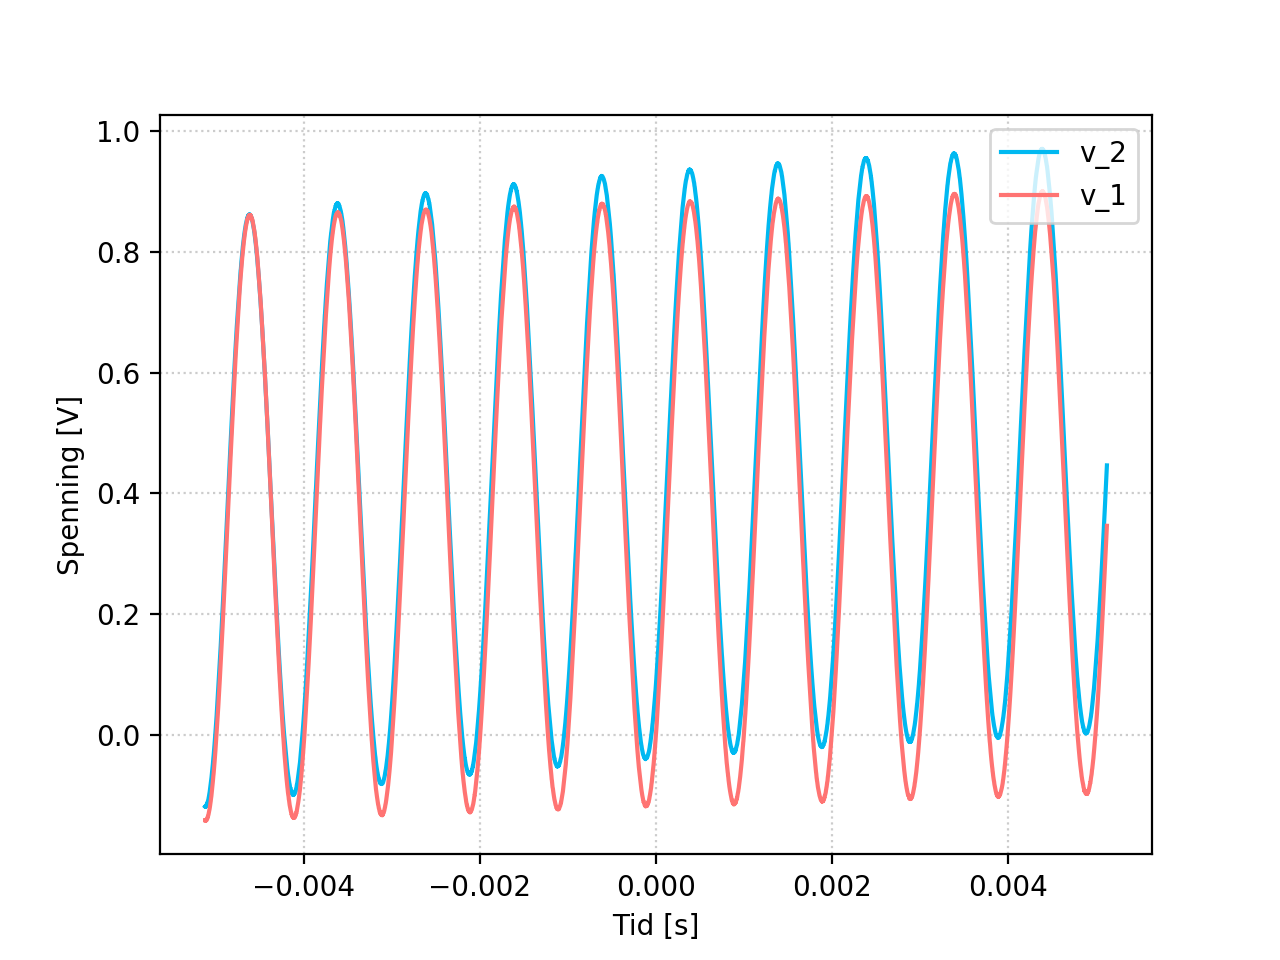
\includegraphics[width=0.8\textwidth]{img/esda2-d5-ideelle-plot.png}
    \caption{Systemet under ideelle forhold.}
    \label{fig:ideal}
\end{figure}
\vspace{1cm}

Amplituden til $v_1$ er $A_1=490\text{mV}$, og amplituden til $v_2$ er $A_2=470\text{mV}$. En ser at $v_2\approx v_1$, som vil si at systemet fungerer godt, men har noe forbedringspotensiale. 

\clearpage

\subsection{Test med reell last og kilde}
En lar $R_\text{L}=220\Omega$ og $R_\text{K}=3.3\text{k}\Omega$. Resultatet av denne addisjonen til systemet vises i figur \ref{fig:real}.

\vspace{1cm}
\begin{figure}[!h]
    \centering
    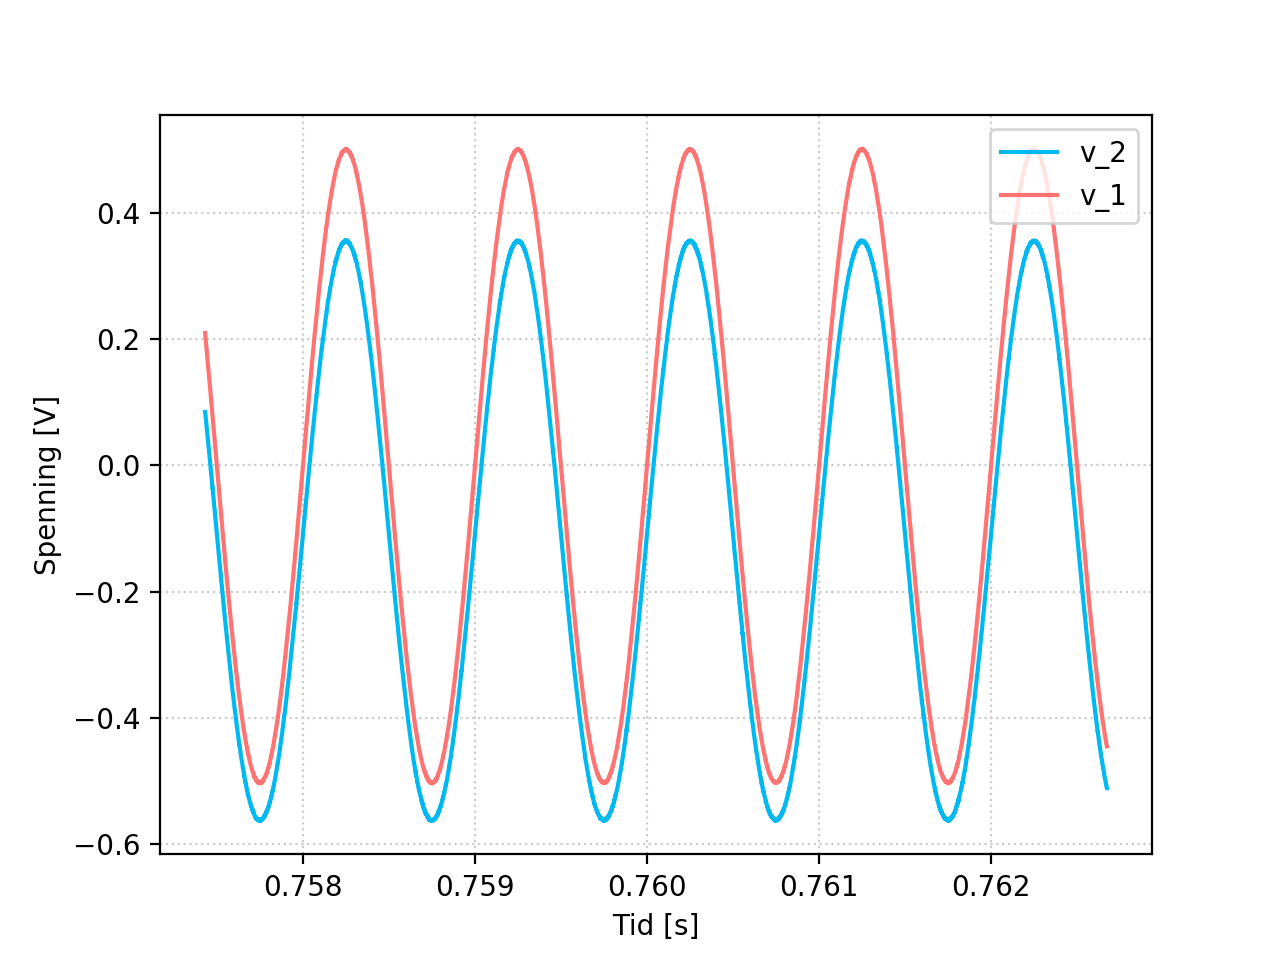
\includegraphics[width=0.8\textwidth]{img/reell-last-kilde.png}
    \caption{Systemet med realistisk last og kilde.}
    \label{fig:real}
\end{figure}
\vspace{1cm}

En finner at $A_2=458\text{mV}$ og $A_1=500\text{mV}$, som vil si at $v_2\approx v_1$, og systemet funker for en reell last og kilde. Den fysiske implementasjonen av kretsen, med reell last og kilde, vises i figur \ref{fig:real-circuit}.

\vspace{1cm}
\begin{figure}[!h]
    \centering
    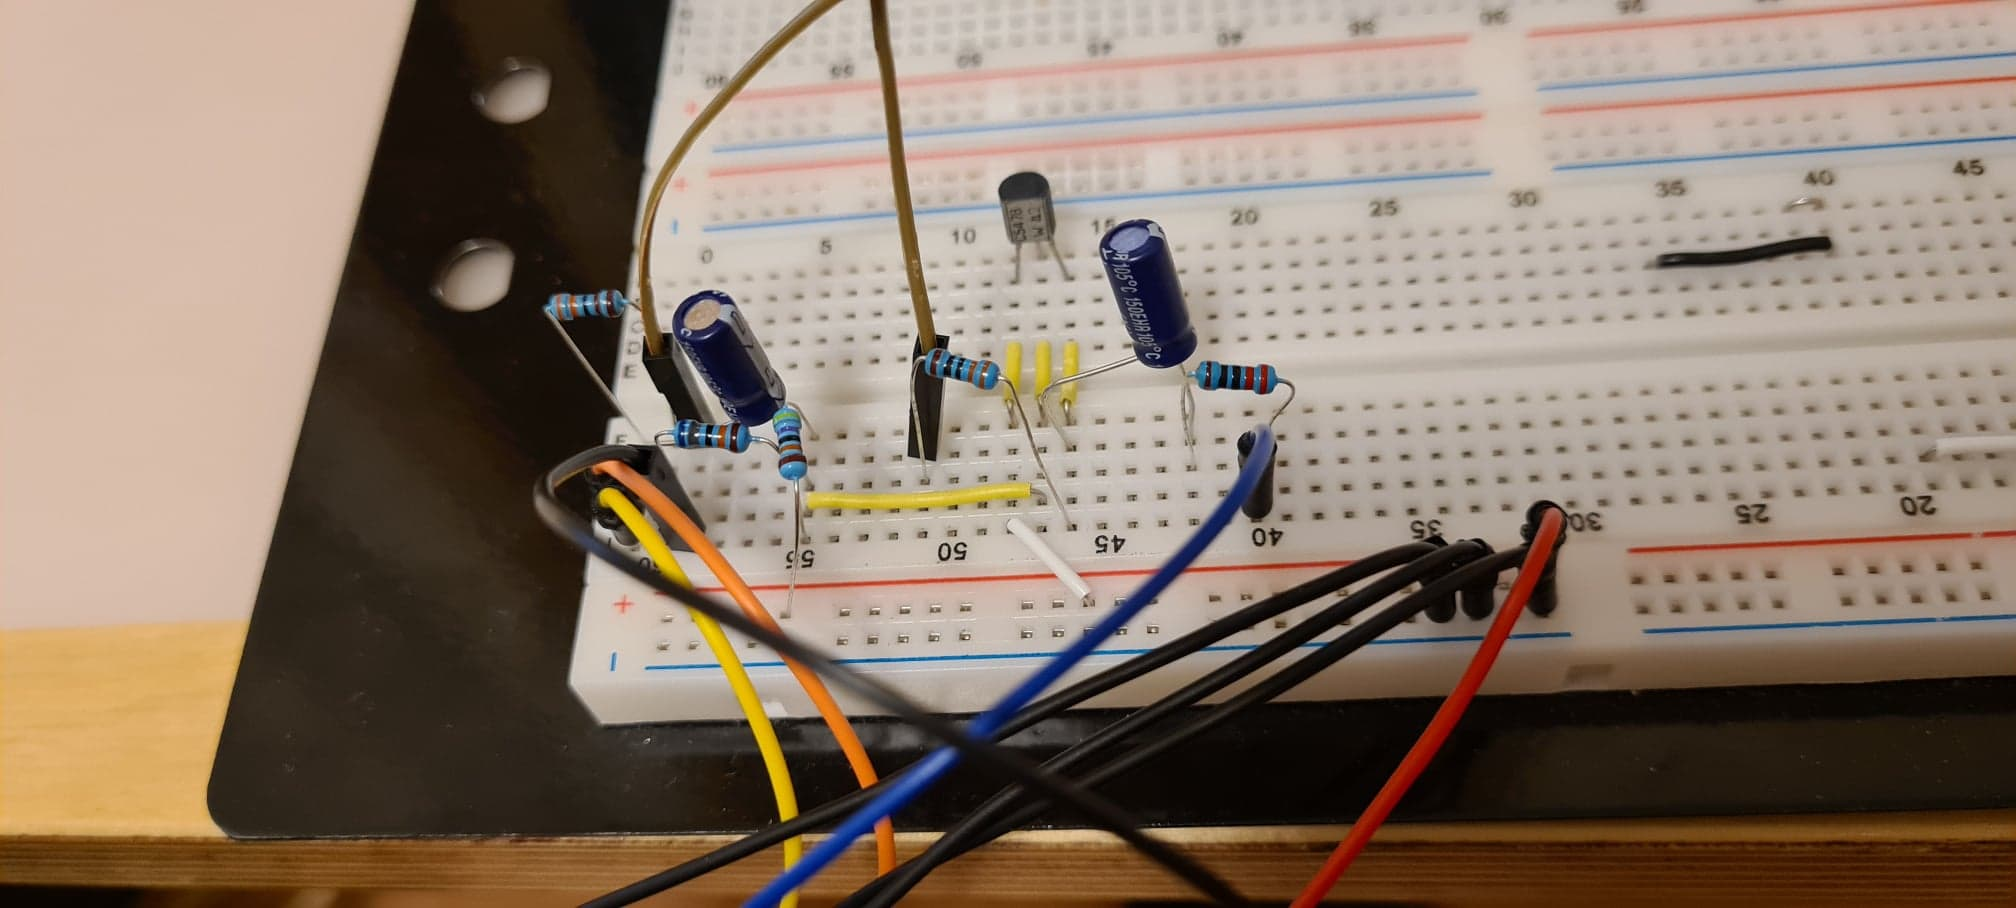
\includegraphics[width=\textwidth]{img/119455020_3605124586185980_8976253010718534837_n.jpg}
    \caption{Det realiserte systemet med realistisk last og kilde.}
    \label{fig:real-circuit}
\end{figure}
\vspace{1cm}

\clearpage


\subsection{Diskusjon}
Systemet ble testa for hvor stor amplitude $v_0$ kan ha før $v_2$ ble klippa, og resultatet vises i figur \ref{fig:v0max}. Der finner en at når $A_1=1\text{V}$, så klippes $v_2$ til $A_2=828\text{mV}$.

\vspace{1cm}
\vspace{1cm}
\begin{figure}[!h]
    \centering
    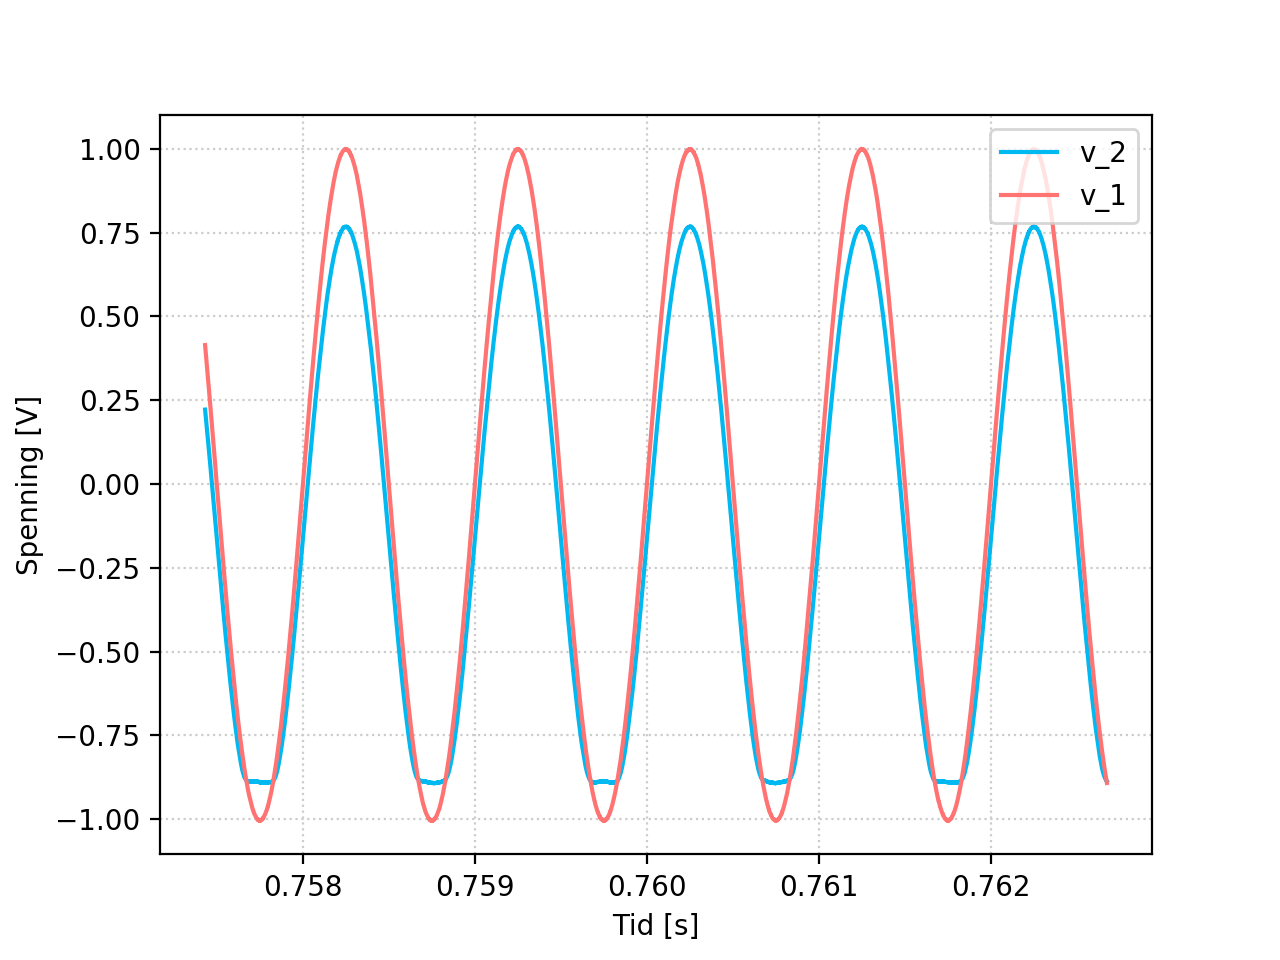
\includegraphics[width=0.8\textwidth]{img/v0max.png}
    \caption{Maksimal amplitude av $v_0$ før $v_2$ klippes.}
    \label{fig:v0max}
\end{figure}
\vspace{1cm}

Verdiene for $R_{\text{B}1}$ og $R_{\text{B}2}$ bestemmer hvor godt systemet funker som en buffer. For at en buffer skal fungere korrekt, så må inngangsimpedansen være høy, og utgangsimpedansen være lav. Verdiene for kondensatorene trenger kun å være tilstrekkelig store i forhold til systemet, og de vil fungere som kortslutninger i en småsignalanalyse (som ikke ble gjort for dette systemet, da en ikke trenger det for å beregne nødvendige komponentverdier).


Frekvensresponsen til systemet vises i figuren under, og en finner at knekkfrekvensen er ved ca. $2\text{MHz}$.

\vspace{1cm}
\begin{figure}[!h]
    \centering
    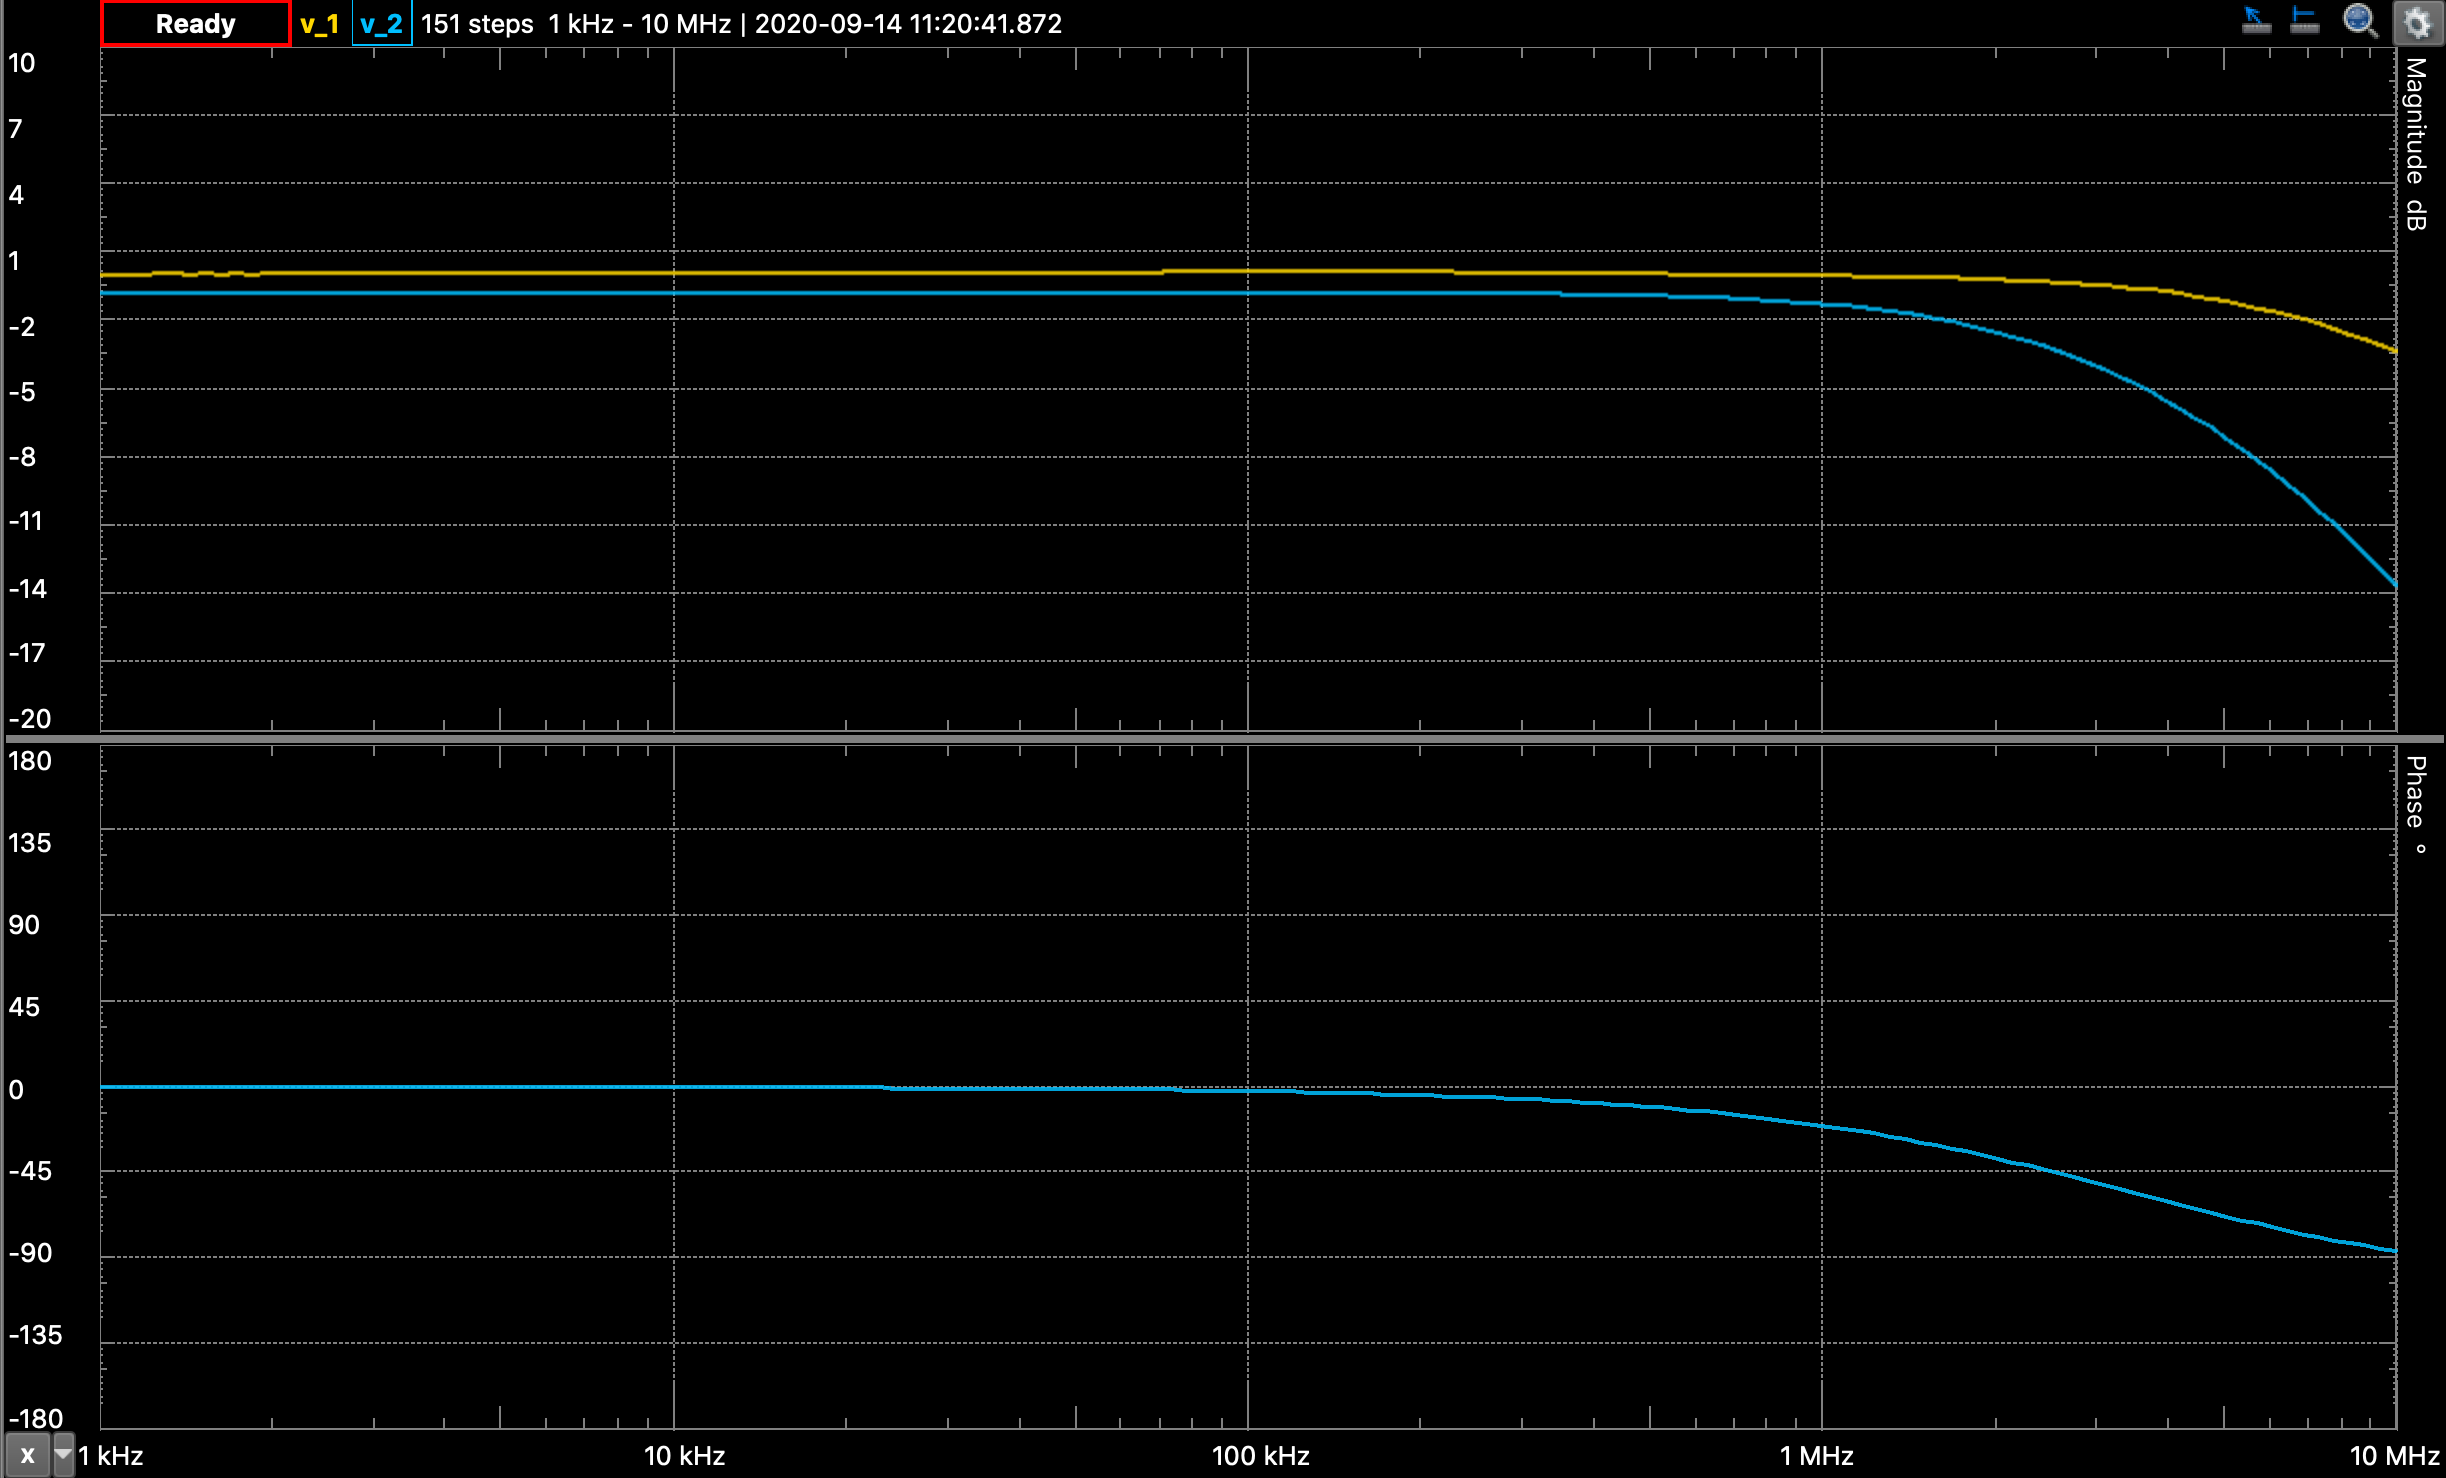
\includegraphics[width=1\textwidth]{img/frekvens-d5.png}
    \caption{Systemets frekvensrespons.}
    \label{fig:f}
\end{figure}
\vspace{1cm}